\documentclass{article}

\usepackage[utf8]{inputenc}
\usepackage[T1]{fontenc}

\usepackage{geometry}
 \geometry{
 a4paper,
 total={170mm,257mm},
 left=20mm,
 top=20mm,
 }

\setlength{\parskip}{7pt}
\setlength{\parindent}{0pt}

\title{RISC-V external debug specification simplified}
\date{2019-09-16}

\usepackage{hyperref}
\usepackage{listings}
\usepackage{amssymb}
\usepackage{graphicx}
\graphicspath{ {./images/} }
\usepackage{float}

\lstset{
	basicstyle=\ttfamily,
	breaklines=true,
	columns=fullflexible,
	tabsize=4,
	showstringspaces=false,
	frame=single
}

\begin{document}
	\maketitle
	
	\section{About}
	
	An official specification for the support of external debugging on RISC-V platforms has been written. At the time of writing, the document is not complete yet. The latest release is \textbf{version 0.13.2} from 2019-03-22.
	
	The release and the working draft are available on Github: \url{https://github.com/riscv/riscv-debug-spec}
	
	This document aims to present the debug architecture and mecanisms in a simplified manner without all the details. Some parts are taken directly from the official specification.
	
	For more detailed explanations, please refer to the official specification.
	
	\newpage
	\section{Overview}
	
	\begin{figure}[H]
   	\centering
   	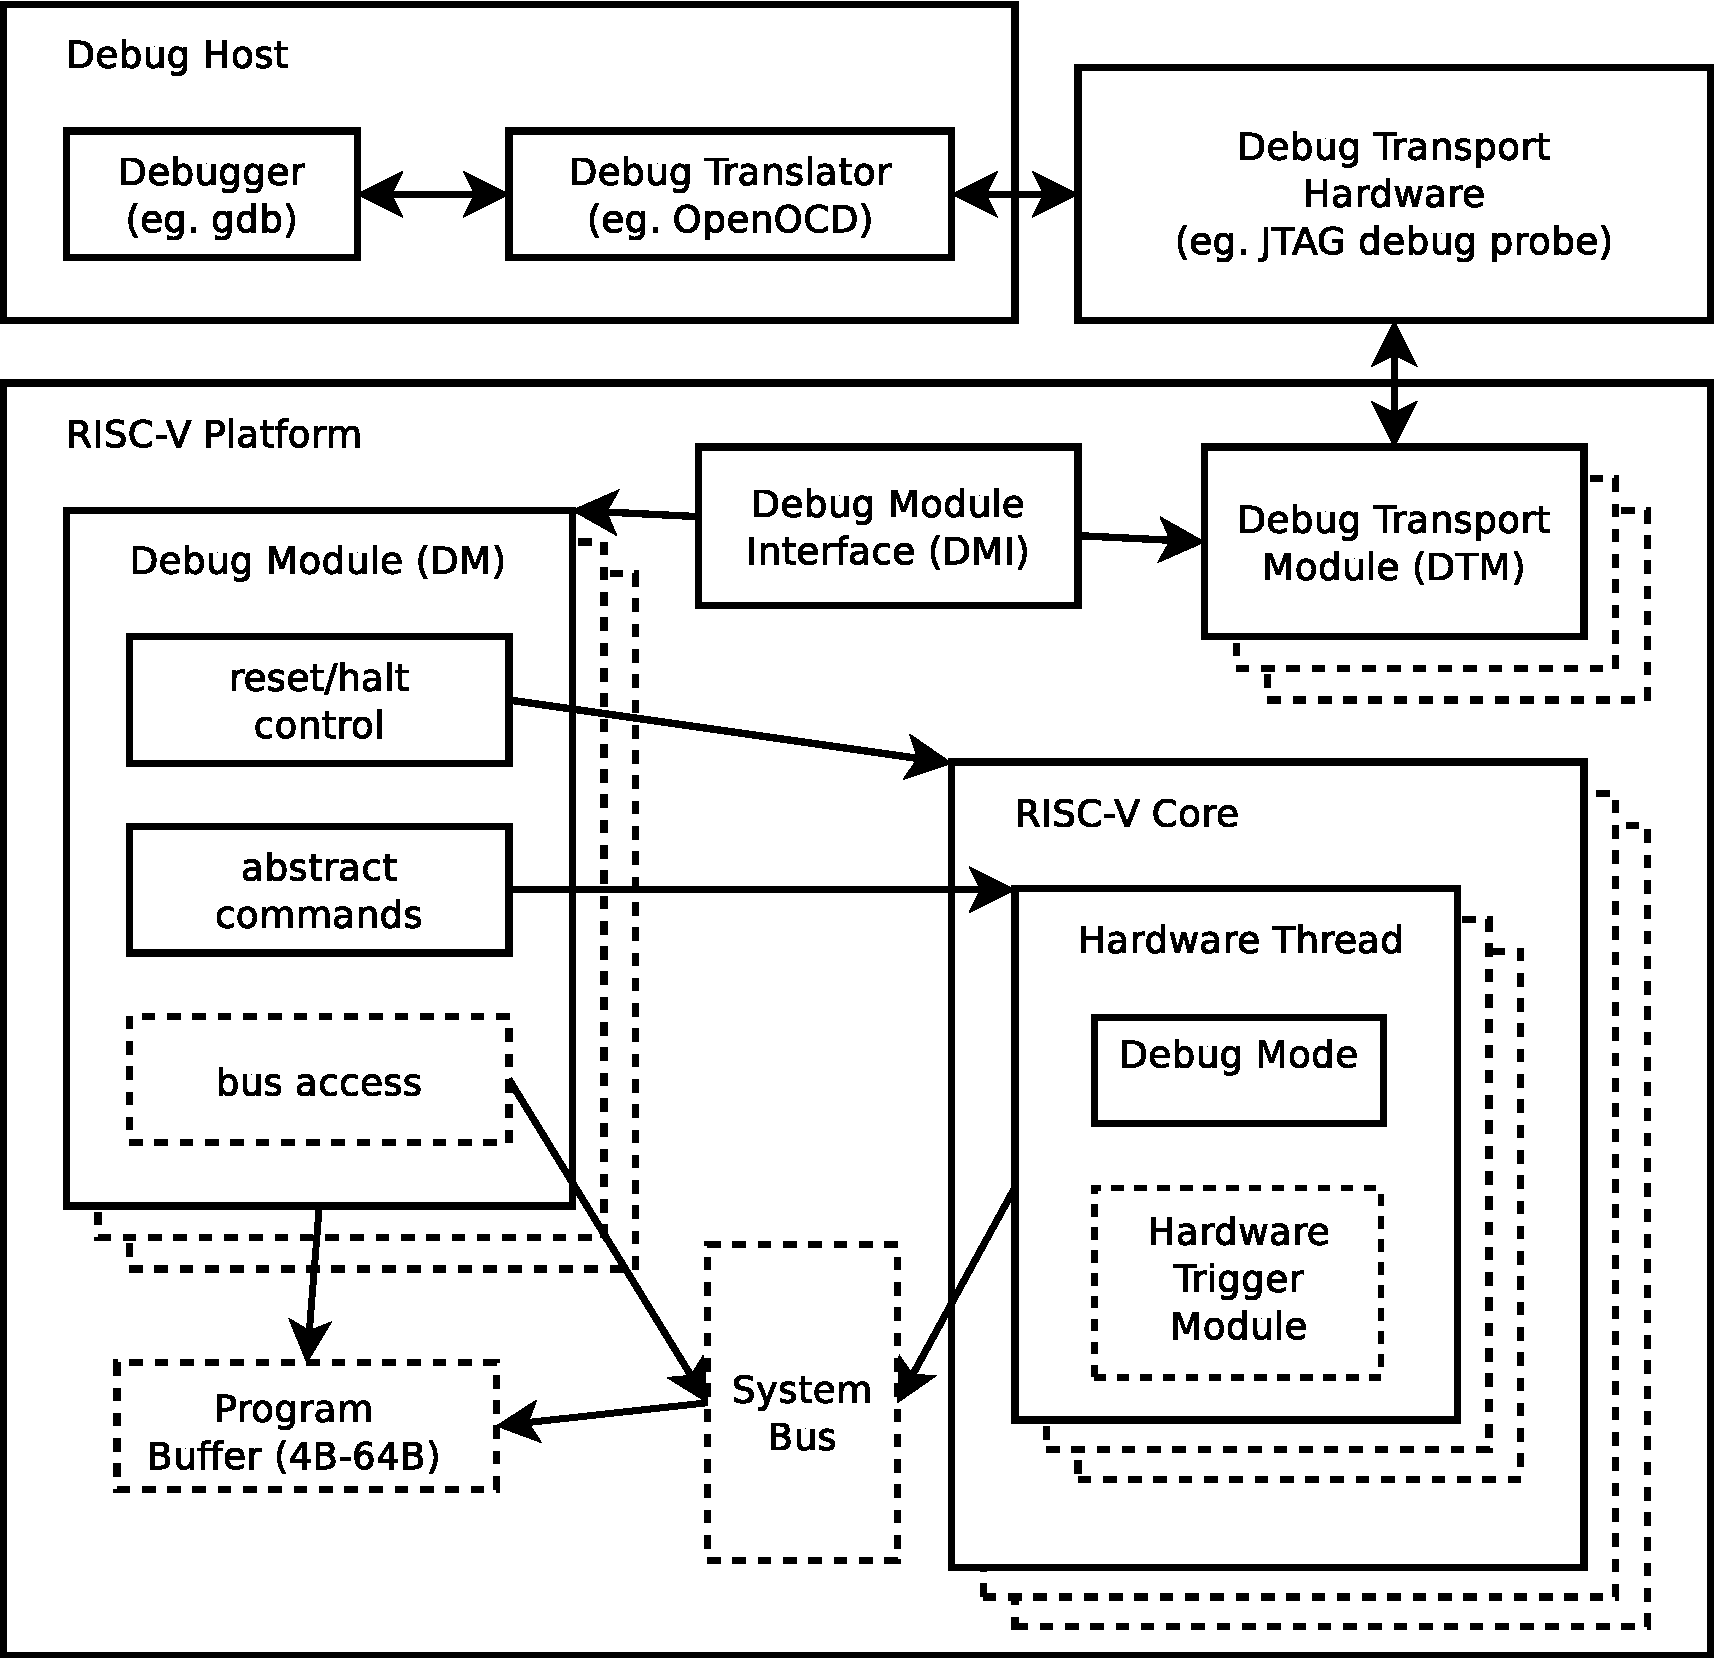
\includegraphics[width=0.82\textwidth]{overview.pdf}
   	\caption{RISC-V Debug System Overview}
   	\label{fig:overview}
	\end{figure}
	
	The system has several elements. The ones that are external to the RISC-V platform are:
	
	\begin{itemize}
	
	\item \textbf{Debugger}: Software to test and debug the target program. gdb is the most popular. A version with RISC-V support can be found as a part of the riscv-gnu-toolchain at \url{https://github.com/riscv/riscv-gnu-toolchain}
	
	\item \textbf{Debug Translator}: Software to translate between the debugger and the platform. OpenOCD is often used. A fork with RISC-V support can be found at \url{https://github.com/riscv/riscv-openocd}
	
	\item \textbf{Debug Transport Hardware}: A way to connect the debug translator to the RISC-V platform. For example, if the system uses JTAG, it could be a JTAG probe.
	
	\end{itemize}
	
	In the RISC-V platform, there are:
	
	\begin{itemize}
	
	\item \textbf{Debug Transport Module (DTM)}: The access point. The DTM provides access to the DM from the exterior.
	
	\item \textbf{Debug Module Interface (DMI)}: A bus that connects the DTM to the DM.
	
	\item \textbf{Debug Module (DM)}: The unit that effectively implements the debug operations. The DM is controlled via register accesses to its DMI address space.
	
	\item \textbf{RISC-V Core}: The part of the platform that performs the instructions and computations. One or several hardware threads (\textbf{harts}) run on it. It can be interrupted and examined by the DM.
	
	\end{itemize}
	
	\newpage
	\section{Debug Transport module (DTM)}
	
	A DTM provides acces to the DMs of the platform. There may be multiple DTMs, but only one can be active at the same time.
	
	The transports used are not specified (e.g. JTAG or USB) and are left to the implementation. Nevertheless, a JTAG DTM has been defined in the specification.
	
	Additional DTMs may be added in future versions of the specification.
	
	\subsection{JTAG DTM}
	
	The JTAG DTM defines a Test Access Port (TAP) that can be accessed using JTAG. The TAP uses the following registers:
	
	\begin{table}[H]
		\begin{center}
			\caption{JTAG DTM TAP Registers}
			\label{dtmTable:jtagregisters}
			\begin{tabular}{|r|l|l|}
			\hline
			Address & Name & Description\\
			\hline
0x00 & BYPASS & JTAG recommends this encoding \\
0x01 & IDCODE & To identify a specific silicon version \\
0x10 & DTM Control and Status ({\tt dtmcs}) & For Debugging\\
0x11 & Debug Module Interface Access ({\tt dmi}) & For Debugging\\
0x12 & Reserved (BYPASS) & Reserved for future RISC-V debugging \\
0x13 & Reserved (BYPASS) & Reserved for future RISC-V debugging \\
0x14 & Reserved (BYPASS) & Reserved for future RISC-V debugging \\
0x15 & Reserved (BYPASS) & Reserved for future RISC-V standards \\
0x16 & Reserved (BYPASS) & Reserved for future RISC-V standards \\
0x17 & Reserved (BYPASS) & Reserved for future RISC-V standards \\
0x1f & BYPASS & JTAG requires this encoding \\
			\hline
			\end{tabular}
		\end{center}
	\end{table}
	
	The \textit{IDCODE} and \textit{BYPASS} registers are standard JTAG registers.
	
	Debug functionnalities are achieved through the \textit{dtmcs} and \textit{dmi} registers.
	
	\subsubsection{DTM Control and Status (dtmcs)}
	
	This register contains:
	
	\begin{itemize}
	
	\item \textbf{Version}: The specification version of the DTM. Possible values are 0.11, 0.13 (current), other.
	
	\item \textbf{Address size}: The size of the addresses used in \textit{dmi}
	
	\item \textbf{Status}: Current status of the DTM (no error, error, busy)
	
	\item \textbf{Reset}: A way to reset or hard-reset the DTM
	
	\end{itemize}
	
	\subsubsection{Debug Module Interface Access (dmi)}
	
	This register is allows access to the DM, through the DMI. It contains:
	
	\begin{itemize}
	
	\item \textbf{Address}: Address used for DMI access
	
	\item \textbf{Data}: The data to write in the DM, or the data to read after an operation
	
	\item \textbf{OP}: The operation (read, write, nop) or the result (success, fail, busy)
	
	\end{itemize}
	
	\newpage
	\section{Debug Module (DM)}
	
	The DM is slave to the DMI. It implements a translation interface between abstract debug operations and their specific implementation.
	
	\subsection{Features}
	
	The DM must support the following features:
	
	\begin{itemize}
	
	\item Give the debugger necessary information about the implementation.
	
	\item Allow any individual hart to be halted and resumed.
	
	\item Provide status on which harts are halted.
	
	\item Provide abstract read and write access to a halted hart’s GPRs (general purpose registers).
	
	\item Provide access to a reset signal that allows debugging from the very first instruction after reset.
	
	\item At least one of these:
		\begin{itemize}
		\item Provide a Program Buffer to force the hart to execute arbitrary instructions.
		\item Allow direct System Bus Access.
		\item Provide abstract access to non-GPR hart registers.
		\end{itemize}
	
	\item At least one of these:
		\begin{itemize}
		\item Implement the Program Buffer
		\item Implement abstract access to all registers that are visible to software running on the hart
		\item Minimal Debug Specification: Implement abstract access to at least all GPRs, \textit{dcsr}, and \textit{dpc}
		\end{itemize}
	
	\end{itemize}
	
	\subsection{Registers}
	
	The multiple functions are realized through the DM registers. These registers are controlled by the DMI.
	
	When read, unimplemented Debug Module DMI Registers return 0. Writing them has no effect.
	
	\begin{table}[H]
   \begin{center}
      \caption{Debug Module Debug Bus Registers}
      \label{dm}
      \begin{tabular}{|r|l|}
      \hline
      Address & Name \\
      \hline
0x04 & Abstract Data 0 ({\tt data0}) \\
0x0f & Abstract Data 11 ({\tt data11}) \\
0x10 & Debug Module Control ({\tt dmcontrol}) \\
0x11 & Debug Module Status ({\tt dmstatus}) \\
0x12 & Hart Info ({\tt hartinfo}) \\
0x13 & Halt Summary 1 ({\tt haltsum1}) \\
0x14 & Hart Array Window Select ({\tt hawindowsel}) \\
0x15 & Hart Array Window  ({\tt hawindow}) \\
0x16 & Abstract Control and Status ({\tt abstractcs}) \\
0x17 & Abstract Command ({\tt command}) \\
0x18 & Abstract Command Autoexec ({\tt abstractauto}) \\
0x19 & Configuration String Pointer 0 ({\tt confstrptr0}) \\
0x1a & Configuration String Pointer 1 ({\tt confstrptr1}) \\
0x1b & Configuration String Pointer 2 ({\tt confstrptr2}) \\
0x1c & Configuration String Pointer 3 ({\tt confstrptr3}) \\
0x1d & Next Debug Module ({\tt nextdm}) \\
0x1f & Custom Features ({\tt custom}) \\
0x20 & Program Buffer 0 ({\tt progbuf0}) \\
0x2f & Program Buffer 15 ({\tt progbuf15}) \\
0x30 & Authentication Data ({\tt authdata}) \\
0x32 & Debug Module Control and Status 2 ({\tt dmcs2}) \\
0x34 & Halt Summary 2 ({\tt haltsum2}) \\
0x35 & Halt Summary 3 ({\tt haltsum3}) \\
0x37 & System Bus Address 127:96 ({\tt sbaddress3}) \\
0x38 & System Bus Access Control and Status ({\tt sbcs}) \\
0x39 & System Bus Address 31:0 ({\tt sbaddress0}) \\
0x3a & System Bus Address 63:32 ({\tt sbaddress1}) \\
0x3b & System Bus Address 95:64 ({\tt sbaddress2}) \\
0x3c & System Bus Data 31:0 ({\tt sbdata0}) \\
0x3d & System Bus Data 63:32 ({\tt sbdata1}) \\
0x3e & System Bus Data 95:64 ({\tt sbdata2}) \\
0x3f & System Bus Data 127:96 ({\tt sbdata3}) \\
0x40 & Halt Summary 0 ({\tt haltsum0}) \\
0x70 & Custom Features 0 ({\tt custom0}) \\
0x7f & Custom Features 15 ({\tt custom15}) \\
         \hline
      \end{tabular}
   \end{center}
\end{table}
	
	\subsection{Run Control}
	
	The DM can control the states of its harts with these registers:
	
	\begin{itemize}
	\item \textbf{dmstatus}: status of the DM and the selected harts
	\item \textbf{dmcontrol}: hart selection, halting and resuming
	\item \textbf{hawindow}: selecting multiple harts
	\item \textbf{hartinfo}: information about the selected harts
	\item \textbf{haltsum0-3}: which harts are halted
	\end{itemize}
	
	\subsection{Program Buffer}
	
	To support executing arbitrary instructions on a halted hart, a Debug Module can include a Program Buffer that a debugger can write small programs to. Systems that support all necessary functionality using abstract commands only may choose to omit the Program Buffer.

	\begin{itemize}
	\item \textbf{progbuf0-15}: the program buffer
	\end{itemize}
	
	\subsection{Abstract Commands}
	
	The DM supports a set of abstract commands:
	
	\begin{itemize}
	\item \textbf{Acces Register}: read or write CPU registers and execute the Program Buffer. R/W access to all GPRs is mandatory; accessing other registers is optional.
	\item \textbf{Quick Access} (optional): halt the hart, execute the Program Buffer, and resume the hart
	\item \textbf{Access Memory} (optional): R/W access in the memory available to the selected hart
	\end{itemize}
	
	The following DM registers are used:
	
	\begin{itemize}
	\item \textbf{abstractcs}: status of abstract commands (free, busy, error)
	\item \textbf{command}: select a command, its arguments, and execute it
	\item \textbf{abstractauto}: autoexecution of commands
	\item \textbf{data0-11}: arguments and return values
	\end{itemize}
	
	\subsection{System Bus Access}
	
	A DM may include a System Bus Access block to provide memory access without involving a hart.
	
	\begin{itemize}
	\item \textbf{sbcs}: status and options
	\item \textbf{sbadress0-3}: set bus address and can trigger a bus read
	\item \textbf{sbdata0-3}: bus data (from a bus read, or for a bus write) and can trigger a bus write
	\end{itemize}
	
	\newpage
	\section{RISC-V Core}
	
	Modifications to the RISC-V core to support debug are kept to a minimum. There is a special execution mode (Debug Mode) and a few extra CSRs. The DM takes care of the rest.
	
	\subsection{Debug Mode}
	
	When a hart is halted for external debugging, it enters Debug Mode.
	
	In Debug Mode, the hart can execute the program Buffer with changes from normal execution:
	
	\begin{itemize}
	\item Machine mode privilege level
	\item All interrupts are masked
	\item Exceptions don't update any registers
	\item Triggers are ignored
	\item Counters and timers may be stopped
	\item Some instructions behave differently
	\item Effective XLEN is DXLEN
	\item Instruction {\tt dret} returns from Debug Mode
	\end{itemize}
	
	\subsection{Core Debug Registers}
	
	The supported Core Debug Registers must be implemented for each hart that can be debugged. They are CSRs, accessible using the RISC-V {\tt csr} opcodes and optionally also using abstract debug commands.
	
	These registers are only accessible from Debug Mode.
	
	\begin{table}[H]
   	\begin{center}
      \caption{Core Debug Registers}
      \label{csr}
      	\begin{tabular}{|r|l|l|}
      	\hline
      	Address & Name \\
      	\hline
0x7b0 & Debug Control and Status ({\tt dcsr}) \\
0x7b1 & Debug PC ({\tt dpc}) \\
0x7b2 & Debug Scratch Register 0 ({\tt dscratch0}) \\
0x7b3 & Debug Scratch Register 1 ({\tt dscratch1}) \\
         \hline
      	\end{tabular}
   	\end{center}
	\end{table}

	\begin{itemize}
	\item \textbf{dcsr}: information about Debug Mode. It is possible to execute a single instruction (single step) by setting a field of this register.
	\item \textbf{dpc}: virtual address of the next instruction to be executed
	\item \textbf{dscratch0-1} (optional): scratch registers that can be used by implementations that need it
	\end{itemize}
	
	\subsection{Trigger Module}
	
	A hart may include a Trigger Module. Triggers can cause a breakpoint exception, entry into Debug Mode, or a trace action without having to execute a special instruction.
	
	\subsubsection{Registers}
	
	The Trigger Module uses registers that are CSRs. They are accessible using the RISC-V {\tt csr} opcodes and optionally also using abstract debug commands
	
	\begin{table}[H]
   \begin{center}
      \caption{Trigger Registers}
      \begin{tabular}{|r|l|}
      \hline
      Address & Name \\
      \hline
0x7a0 & Trigger Select ({\tt tselect}) \\
0x7a1 & Trigger Data 1 ({\tt tdata1}) \\
0x7a1 & Match Control ({\tt mcontrol}) \\
0x7a1 & Instruction Count ({\tt icount}) \\
0x7a1 & Interrupt Trigger ({\tt itrigger}) \\
0x7a1 & Exception Trigger ({\tt etrigger}) \\
0x7a2 & Trigger Data 2 ({\tt tdata2}) \\
0x7a3 & Trigger Data 3 ({\tt tdata3}) \\
0x7a4 & Trigger Info ({\tt tinfo}) \\
         \hline
      \end{tabular}
   \end{center}
	\end{table}
	
	\begin{itemize}
	\item \textbf{tselect}: select a trigger
	\item \textbf{tdata1-3}: trigger type and type-specific data
	\item \textbf{mcontrol}: operations for address/data match triggers
	\item \textbf{icount}: operations for instruction count triggers
	\item \textbf{itrigger}: operations for interrupt triggers
	\item \textbf{etrigger}: operations for exception triggers
	\item \textbf{tinfo}: information about supported trigger types
	\end{itemize}
	
	
\end{document}
